\documentclass{article}
\usepackage{amsmath, amsfonts, amssymb, amsthm}
\usepackage{graphicx}
\usepackage{tikz}
\usepackage{listings}

\usepackage{listings}
\usepackage{xcolor}

\lstdefinestyle{custompython}{
  language=Python,
  basicstyle=\ttfamily\small,
  keywordstyle=\color{blue},
  stringstyle=\color{red},
  commentstyle=\color{green},
  breaklines=true,
  breakatwhitespace=true,
  showstringspaces=false,
  numbers=left,
  numberstyle=\tiny,
  frame=single
}

\title{Passive Optical Network Planning}
\date{}
\usepackage{tikz}
\usetikzlibrary{shapes.geometric,arrows.meta}
\begin{document}
\maketitle

\section{Introduction}
Passive Optical Networks (PONs) are systems that use point-to-multipoint fiber to the premises in which unpowered optical splitters are used to enable a single optical fiber to serve multiple endpoints. Designing a cost-effective and efficient PON is critical to ensure optimal performance and investment returns.

\section{Problem Statement}
Given a distribution network, the objective is to plan the optimal placement of splitters and the routing of fibers in such a way that the total network cost is minimized. 

\subsection{Specifications}
\begin{itemize}
    \item The central office is represented by squares and serves as the main connection hub.
    \item Optical Network Units (ONUs) are endpoints represented by circles (type).
    \item Splitters have a fixed capacity of 32 and are represented by triangles (type).
    \item The network graph is provided, which outlines the potential placement locations for splitters and the links (edges) connecting them.
    \item Each edge (fiber) has a cost per meter.
    \item Digging trenches has an associated cost.
    \item It is possible to lay multiple fibers in a single trench, termed as fiber duct sharing.
    \item Each splitter has an associated cost.
\end{itemize}

\subsection{Decision Variables}
\begin{itemize}
    \item \( y_{s} \) : Binary decision variable which is 1 if splitter \( s \) is selected and 0 otherwise.
    \item \( x_{e} \) : Binary decision variable which is 1 if edge \( e \) is selected and 0 otherwise.
\end{itemize}

\subsection{Objective}
Minimize the total cost, which includes the cost of selected splitters, the cost of laying fiber on selected edges, and the trenching cost.

\section{Data}

\begin{lstlisting}[style=custompython, caption=Python Code for PON Model]
model pon

end

import elytica
import json
file = open('gars6.json')
graph = json.load(file)

edges = [{**item, 'nid': index} for index, item in enumerate(graph["edges"])]
nodes = [{**item, 'nid': index} for index, item in enumerate(graph["nodes"])]
loadSplitters = lambda: [n['nid']  for n in nodes if n['type'] == 'triangle']
loadONUs = lambda: [n['nid']  for n in nodes if n['type'] == 'circle']
loadIntermediate = lambda: [n['nid']  for n in nodes if n['type'] == None]
loadCOs = lambda: [n['nid']  for n in nodes if n['type'] == 'square']
loadCommodities = lambda: loadONUs() + loadSplitters()
loadVertices = lambda: [n['nid'] for n in nodes]
loadEdges = lambda: [a['nid'] for a in edges]
loadM = len(edges) * 2
def generateArcs(edges):
  edge_len = len(edges)
  return [
    {
      'weight': edge['weight'],
      'source': direction[0],
      'target': direction[1],
      'id': edge['id'] + suffix,
      'label': edge['label'],
      'nid': edge['nid'] if index == 0 else edge['nid'] + edge_len
    }
    for edge in edges
    for index, (direction, suffix) in enumerate([((edge['source'], edge['target']), '-1'), ((edge['target'], edge['source']), '-2')])
  ]

arcs = generateArcs(edges)
loadArcs = lambda: [a['nid'] for a in arcs]
loadIncomming = lambda: {n['nid']: [a['nid'] for a in arcs if a['target'] == n['id']] for n in nodes}
loadOutgoing = lambda: {n['nid']: [a['nid'] for a in arcs if a['source'] == n['id']] for n in nodes}
loadArcWeights = lambda: {a['nid']:a['weight'] for a in arcs}
loadNodeCosts = lambda: {n['nid']: 0 if not n['modules'] else n['modules'][0]['cost'] for n in nodes}


# Calculate the midpoint
mid_x = sum(node["x"] for node in nodes) / len(nodes)
mid_y = sum(node["y"] for node in nodes) / len(nodes)

# Translate the nodes relative to the midpoint
translated = [{"x": node["x"] - mid_x, "y": node["y"] - mid_y} for node in nodes]

# Find the scaling range
min_x, max_x = min(node["x"] for node in translated), max(node["x"] for node in translated)
min_y, max_y = min(node["y"] for node in translated), max(node["y"] for node in translated)

def get_color(node):
  if node["type"] == 'triangle':
    return '#0000ff'
  if node["type"] == 'square':
    return '#00ff00'
  if node["type"] == 'circle':
    return '#ff0000'
  return '#000000'

def main():
  solve = False # False will render the input

  visual_vertices = [{
    **node, 
    "x": ((node["x"] - mid_x - min_x) / (max_x - min_x or 1)) * 500,
    "y": ((node["y"] - mid_y - min_y) / (max_y - min_y or 1)) * 500,
    "name": node["id"],
    "symbol": node["type"],
    "symbolSize": node["size"],
    "itemStyle": {"color": node["color"] if node["color"] is not None else get_color(node)},
    "id": None
   } for node in nodes]
  visual_edges = [{
    **edge, 
    "id": None,
    "weight": None,
    "label": None,
    "symbol": None
   } for edge in edges]
  visual_vertices = [{k: v for k, v in node.items() if v is not None} for node in visual_vertices]
  visual_edges = [{k: v for k, v in edge.items() if v is not None} for edge in visual_edges]
  if solve:
    elytica.init_model("pon")
    elytica.run_model("pon")
    # visualize the resulting datasets with the following:
    #resulting_edges = [ e for e in elytica.get_model_set("pon", "E")  if elytica.get_variable_value("pon", f"x{e}") > 0.5 ]
    #resulting_splitters = [ s for s in elytica.get_model_set("pon", "S")  if elytica.get_variable_value("pon", f"y{s}") > 0.5 ]
    #no_splitters = [v for v in visual_vertices if ('type' not in v) or (v['type'] != 'triangle')]
    #splitters = [v for v in visual_vertices if v['nid'] in resulting_splitters]
    #visual_vertices  = splitters + no_splitters
    #visual_edges = [e for e in visual_edges if e['nid'] in resulting_edges]

  chart = {
    "series": [ {
      "roam": 'zoom',
      "type": 'graph',
      "layout": 'none',
      "data": visual_vertices,
      "edges": visual_edges,
      "lineStyle": {
        "opacity": 1,
        "width": 3
        }
      }
    ],
   }


  elytica.write_results(json.dumps({"chart": chart})) 
  return 0

\end{lstlisting}

Participants will be provided with a starting code (as shown above) which includes a JSON data structure containing the network graph.

\section{Evaluation}
Solutions will be evaluated based on the following criteria:
\begin{itemize}
    \item Correctness: Does the solution respect all given constraints?
    \item Optimality: How close is the solution to the optimal cost?
    \item Computational Efficiency: How efficiently does the solution run?
\end{itemize}

\section{Submission Guidelines}
Participants are encouraged to use Mixed-Integer Linear Programming (MILP) via Elytica to address the problem. However, if heuristics are employed, the implementation should be compilable on a Unix-based machine. For those using proprietary MIP solvers, a .lp file must be provided, which will be executed using HiGHS. All relevant code and results should be included in the submission.

\section{Datasets}
The intricacies of a JSON-formatted dataset are outlined in Listing \ref{lst:jsonstructure}. The dataset consists of two primary entities: \texttt{edges} and \texttt{nodes}.

Each \texttt{edge} represents a potential location for placing a fiber and is characterized by several attributes. The \texttt{weight} of an edge indicates its length. The unit cost of trenching is R150 per meter, while the cost of fiber is R50 per meter. This is used to calculate the total cost for each edge based on its length. Additionally, each edge has details about its starting point (\texttt{source}), endpoint (\texttt{target}), and a unique identifier (\texttt{id}).

The \texttt{nodes} encapsulate distinct network components with specified functionalities:
\begin{itemize}
    \item CO (Central Office) nodes are symbolized as squares, acting as the primary hubs for telecommunications.
    \item Triangles pinpoint potential locations for splitters which, when positioned, would be responsible for distributing optical signals.
    \item ONUs (Optical Network Units) are visualized as circles and act as service subscriber endpoints in the network.
    \item Intermediate nodes, which might serve as routing points or simple connection hubs, don't have a distinct type but remain essential for maintaining the network's connectivity.
\end{itemize}



\begin{lstlisting}[basicstyle=\ttfamily, frame=single,caption={JSON Structure},label=lst:jsonstructure]
{
    "edges": [
        {
            "weight": ...,
            "source": ...,
            "id": ...,
            "label": ...,
            "target": ...
        },
        ...
    ],
    "nodes": [
        {
            "color": ...,
            "size": ...,
            "modules": [
                {
                    "cost": ...,
                    "capacity": ...
                },
                ...
            ],
            "id": ...,
            "x": ...,
            "type": ...,
            "label": ...,
            "y": ...
        },
        ...
    ]
}
\end{lstlisting}
Figure \ref{fig:micronet} offers a visual representation of the \texttt{micronet.json} dataset, showcasing the interconnectedness of the nodes. The specific shape of each node allows for immediate identification of its role within the network, while the edges, underscore potential pathways for fiber and their corresponding lengths.
\begin{figure}[!ht]
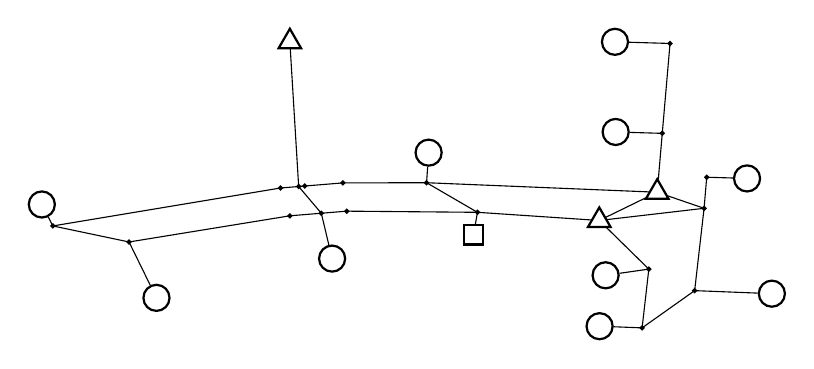
\begin{tikzpicture}
\begin{scope}[every node/.style={scale=0.5,regular polygon,regular polygon sides = 3,thick,draw}]
\node (LOC-1406) at (7.815450,1.722650) {};
\node (LOC-1408) at (7.079600,1.363850) {};
\node (LOC-4252) at (3.149950,3.632800) {};
\end{scope}\begin{scope}[every node/.style={circle, thick, draw}]
\node (LOC-785) at (7.279050,3.632800) {};
\node (LOC-786) at (7.287650,2.488000) {};
\node (LOC-787) at (8.956400,1.897900) {};
\node (LOC-794) at (7.160100,0.667800) {};
\node (LOC-795) at (7.083550,0.021250) {};
\node (LOC-797) at (9.271550,0.434450) {};
\node (LOC-900) at (4.912350,2.225300) {};
\node (LOC-928) at (0.000000,1.567200) {};
\node (LOC-934) at (1.455900,0.381100) {};
\node (LOC-941) at (3.686500,0.879800) {};
\end{scope}\begin{scope}[every node/.style={circle, thick, draw, scale=0.1}]
\node (LOC-1405) at (8.410500,1.518500) {};
\node (LOC-3018) at (5.532400,1.467600) {};
\node (LOC-3031) at (3.031000,1.776300) {};
\node (LOC-3032) at (3.149950,1.423200) {};
\node (LOC-3034) at (3.872550,1.482300) {};
\node (LOC-3035) at (3.823850,1.841150) {};
\node (LOC-4095) at (7.978150,3.611950) {};
\node (LOC-4096) at (7.879500,2.470350) {};
\node (LOC-4097) at (8.444100,1.913150) {};
\node (LOC-4104) at (7.708700,0.746200) {};
\node (LOC-4105) at (7.623650,-0.000000) {};
\node (LOC-4107) at (8.290850,0.472950) {};
\node (LOC-4210) at (4.886300,1.843350) {};
\node (LOC-4238) at (0.140100,1.294500) {};
\node (LOC-4248) at (1.107700,1.090800) {};
\node (LOC-4249) at (3.339250,1.801550) {};
\node (LOC-4250) at (3.261950,1.795200) {};
\node (LOC-4251) at (3.549350,1.455900) {};
\end{scope}\begin{scope}[every node/.style={scale=0.75,regular polygon,regular polygon sides = 4,thick,draw}]
\node (LOC-1158) at (5.482900,1.182800) {};
\end{scope}
\begin{scope}[>={Stealth[black]}, every node/.style={fill=none}, every edge/.style={draw=black}]
\path [-] (LOC-3018)edge node {} (LOC-1158);
\path [-] (LOC-1406)edge node {} (LOC-4210);
\path [-] (LOC-3031)edge node {} (LOC-4238);
\path [-] (LOC-3032)edge node {} (LOC-4248);
\path [-] (LOC-3035)edge node {} (LOC-4210);
\path [-] (LOC-3034)edge node {} (LOC-3018);
\path [-] (LOC-1405)edge node {} (LOC-1406);
\path [-] (LOC-1408)edge node {} (LOC-1405);
\path [-] (LOC-1406)edge node {} (LOC-1408);
\path [-] (LOC-785)edge node {} (LOC-4095);
\path [-] (LOC-786)edge node {} (LOC-4096);
\path [-] (LOC-787)edge node {} (LOC-4097);
\path [-] (LOC-794)edge node {} (LOC-4104);
\path [-] (LOC-795)edge node {} (LOC-4105);
\path [-] (LOC-797)edge node {} (LOC-4107);
\path [-] (LOC-900)edge node {} (LOC-4210);
\path [-] (LOC-928)edge node {} (LOC-4238);
\path [-] (LOC-934)edge node {} (LOC-4248);
\path [-] (LOC-941)edge node {} (LOC-4251);
\path [-] (LOC-3018)edge node {} (LOC-1408);
\path [-] (LOC-4095)edge node {} (LOC-4096);
\path [-] (LOC-4096)edge node {} (LOC-1406);
\path [-] (LOC-1405)edge node {} (LOC-4097);
\path [-] (LOC-1408)edge node {} (LOC-4104);
\path [-] (LOC-4104)edge node {} (LOC-4105);
\path [-] (LOC-4107)edge node {} (LOC-1405);
\path [-] (LOC-3035)edge node {} (LOC-4249);
\path [-] (LOC-4249)edge node {} (LOC-4250);
\path [-] (LOC-4250)edge node {} (LOC-3031);
\path [-] (LOC-3032)edge node {} (LOC-4251);
\path [-] (LOC-4251)edge node {} (LOC-3034);
\path [-] (LOC-4238)edge node {} (LOC-4248);
\path [-] (LOC-4107)edge node {} (LOC-4105);
\path [-] (LOC-4251)edge node {} (LOC-4250);
\path [-] (LOC-4210)edge node {} (LOC-3018);
\path [-] (LOC-4252)edge node {} (LOC-4250);
\end{scope}
\end{tikzpicture}
\caption{micronet.json visualized.}\label{fig:micronet}
\end{figure}

\begin{center}
\textbf{Competition Rules}
\end{center}

\begin{enumerate}
    \item \textbf{No Team Participation}: This is an individual competition. Team submissions will not be accepted.
    \item \textbf{Time Limit}: Participants are given a strict time limit of 2 hours from the start of the competition to finalize and submit their solutions.
    \item \textbf{Assistance}: The Elytica team will be available to assist with the Elytica syntax and general programming errors. However, they will not provide any assistance with model formulation.
    \item \textbf{Submission}: Participants should email their script or code, along with the model formulation, to \texttt{info@elytica.com} before the deadline.
    \item \textbf{Resources}: Participants are welcomed to make use of any online resources to aid their work during the competition. However, all work submitted must be original and not copied from other sources.
\end{enumerate}
\end{document}
